\chapter{Aufbau: Erweiterung der Filterkombinationen}
\thispagestyle{fancy}

Im Zuge dieser Arbeit wurden für eine Erhöhung der Messpunkte und Verringerung von Rauschen bei der leistungsdichteabhängigen Messung der IQE die Anzahl der Filterkombination erhöht. Dafür wurden die alten zwei Filterräder durch drei neue ersetzt. 
%
\begin{figure}[ht!]
    \centering
    \begin{minipage}[t]{1\linewidth}
        \centering
        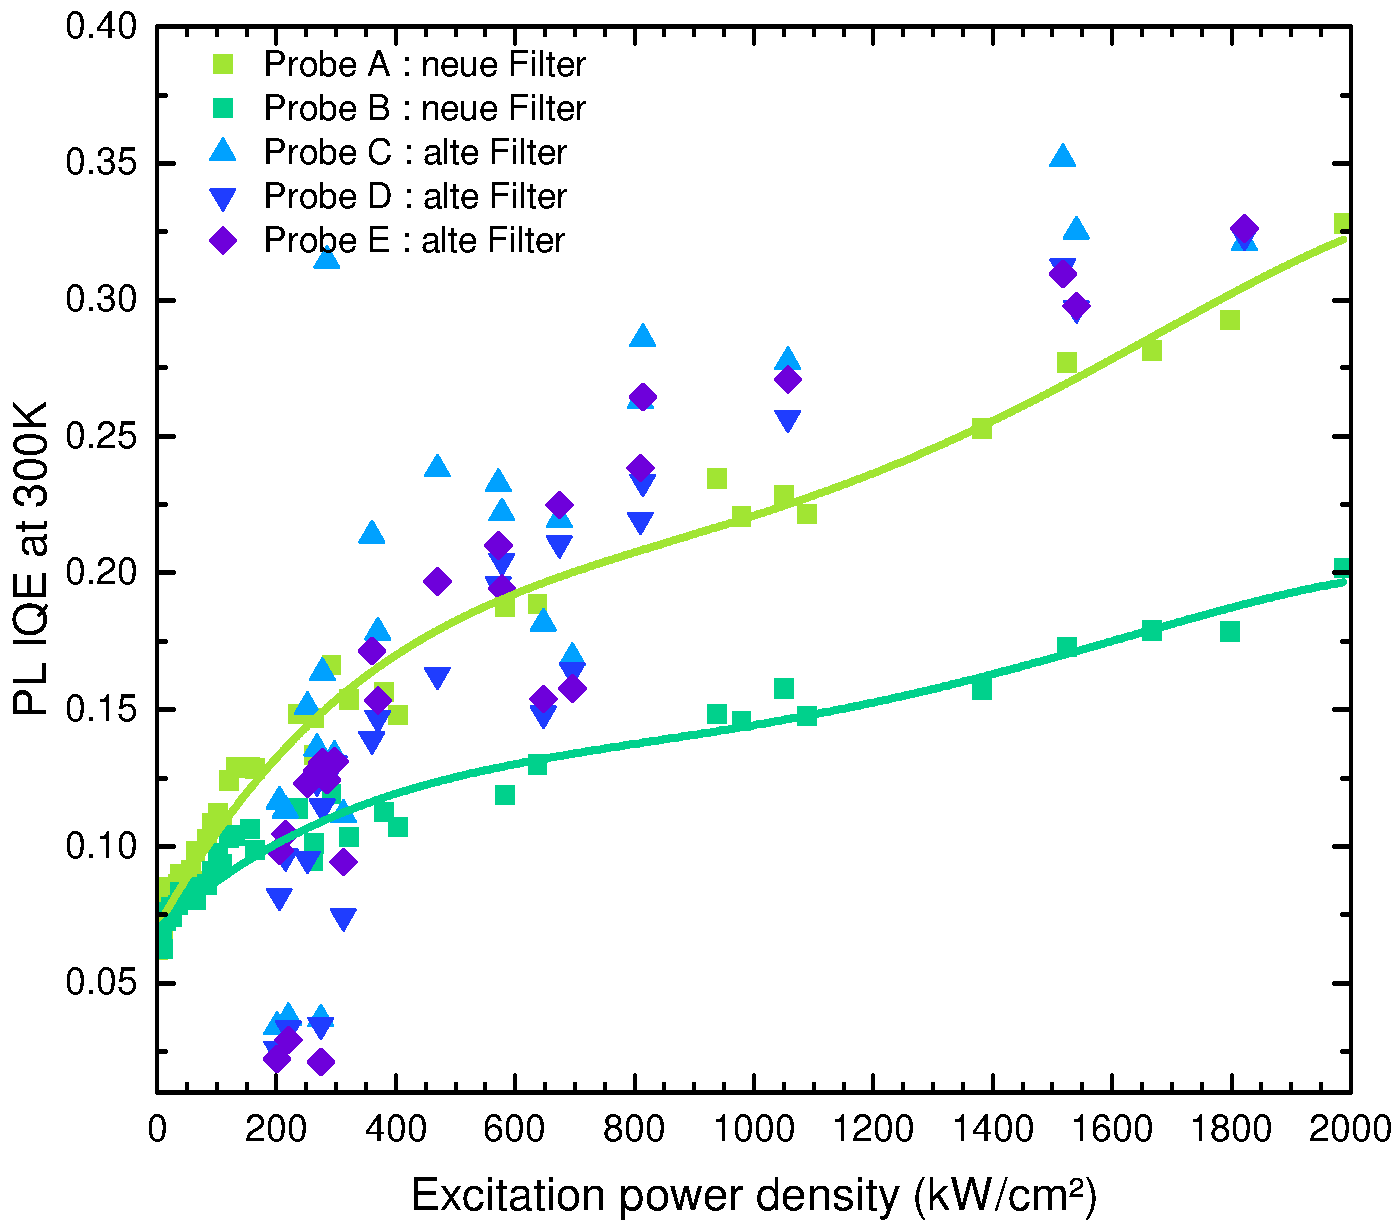
\includegraphics[width = 0.5\linewidth]{Bilder/AuswertungNovemeberKorr1VergleichFilter.pdf}
        \caption{Vergleich der Messung von insgesamt 5 ähnlichen Proben. 3 Proben (grün) wurden mit dem alten Setup gemessen. 2 Proben (blau, durchgezogene Linie) wurden mit dem neuen Setup gemessen. Die Präzision in tieferen Anregungsleistungsdichtenbereichen ist für das neue Setup deutlich erhöht. Das Rauschen fällt ebenfalls deutlich geringer aus. }
        \label{fig:vergleichFilter}
    \end{minipage}
\end{figure}
%
\newpage
Durch die erhöhte Anzahl möglicher Filterkombinationen ist es mit diesen möglich, statt nur 27 verschiedenen Messpunkte 61 zu nehmen. Speziell der Bereich der geringen Anregungsleistungsdichten kann so besser aufgelöst werden und das Rauschen wurde im Allgemeinen stark verringert. 
Wie in Abb \ref{fig:vergleichFilter} zu sehen ist, haben wir durch die Erhöhung der Filterkombinationen speziell im Bereich geringerer Anregungsleistungsdichten weniger Rauschen. Nun ist es möglich, mit der Anregungsleistungsdichte deutlich tiefer zu gehen. Zusätzlich wird die Anregungsleistungsdichte nun auch während des Experiments vermessen, um den Einfluss der Laserschwankung zu verringern, die abhängig ist von der Dauer des Betriebs, der Gasbefüllung und Umgebungstemperatur des Lasers. 
